This section presents the results of the tests conducted on the simulated data. The tests include the marginal model test, the neural copula test, and the portfolio test, defined in \Cref{sec:Method}.

\subsection{Marginal Model Test}
The losses of the models in the marginal model test after training is shown in \Cref{tab:MarginalFinalLosses}. The table shows the total loss and the losses for each of the four terms in the loss function. The total loss is the sum of the four terms. The loss terms L2, L3, and L4 are the losses governed by constraints whereas L1 is the term maximizing the likelihood of the observed data. 

We can see that constraint losses are very close to zero for all distributions, indicating that the models satisfy the constraints. In \Cref{fig:MarginalResults}, we show the trained \gls{CDF} in a plot together with its corresponding \gls{PDF} and the observed data in a histogram. The generated QQ plots all show a perfect straight line and hence the inclusion of these plots is omitted. Visually it seems like the fitted models are able to capture the true distributions well. The most difficult distribution to fit seems to be the uniform distribution which has a somewhat unstable \gls{PDF}, this is also reflected in the total loss being the greatest. Overall, all distributions seem to be fitted well, and the QQ plots indicate that the transformed data is very similar regardless of whether using the fitted model or the true distribution. The conclusion is that the marginal model seem to be able to adequately fit a wide range of distributions. The results of the marginal model test answer the first research question \RQone about if the marginal models are adequate for the task of fitting the marginal distributions. The answer to this question is yes as the models are able to fit the distributions well. These results are limited to the distributions tested and the data used. The models may not perform as well on other distributions or datasets. There is however, nothing in these results suggest that the results would not hold. These results are in line with the results of \Citet[FindPage]{ZengWang2022}. What would be interesting to see is how to best work around the requirement of having to normalize the data before training the marginal models. This becomes especially relevant when trying to fit distributions that accurately capture the tails of the distribution where observations are rare.  


\begin{table}[h]
    \centering
    \caption{Losses for the trained marginal models after training for each distribution.}
    \begin{tabular}{llllll}
        Distribution & Total Loss & L1 & L2 & L3 & L4 \\
        \midrule
        Gaussian & -0.610431 & -0.6109432 & 0.0 & 0.00030577183 & 0.000206 \\
        Student-t & -1.700450 & -1.7008212 & 0.0 & 0.00023537874 & 0.000135 \\
        Uniform & 0.002953 & 0.0013246911 & 0.0 & 0.0008457899 & 0.000782 \\
        Exponential & -1.148577 & -1.1511308 & 0.0 & 0.0011827946 & 0.001371 \\
        Laplace & -1.196009 & -1.1963692 & 0.0 & 0.00022995472 & 0.000130 \\
        LogNormal & -2.257325 & -2.2578392 & 0.0 & 0.0002965927 & 0.000218 \\
    \end{tabular}
    \label{tab:MarginalFinalLosses}
\end{table}


\begin{figure}
    % --- (a) Normal ---
        \begin{minipage}{0.45\textwidth}
            \centering
            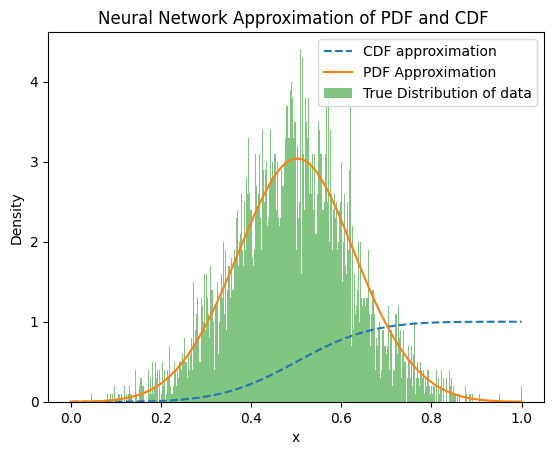
\includegraphics[width=\textwidth]{5ResultsDiscussion/pictures/MarginalTest/NormalHistogram.png}
            \subcaption*{(a) Normal}
        \end{minipage}
    \hfill
    % --- (b) Student's t ---
        \begin{minipage}{0.45\textwidth}
            \centering
            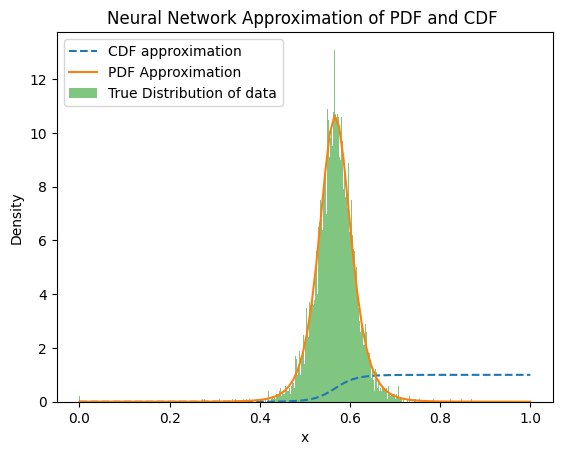
\includegraphics[width=\textwidth]{5ResultsDiscussion/pictures/MarginalTest/StudentsHistogram.png}
            \subcaption*{(b) Student's t}
        \end{minipage}

    \vspace{1em}

    % --- (c) Uniform ---
        \begin{minipage}{0.45\textwidth}
            \centering
            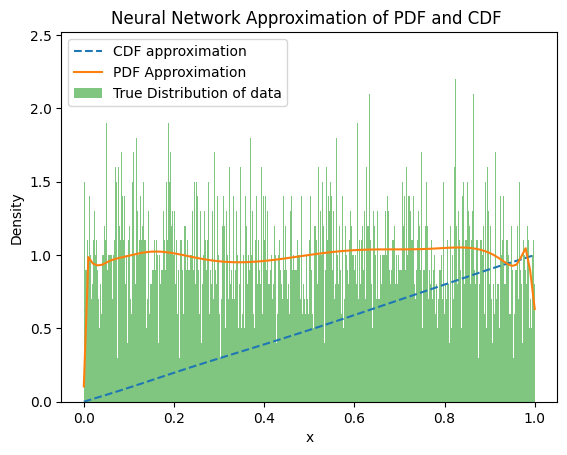
\includegraphics[width=\textwidth]{5ResultsDiscussion/pictures/MarginalTest/UniformHistogram.png}
            \subcaption*{(c) Uniform}
        \end{minipage}
    \hfill
    % --- (d) Exponential ---
        \begin{minipage}{0.45\textwidth}
            \centering
            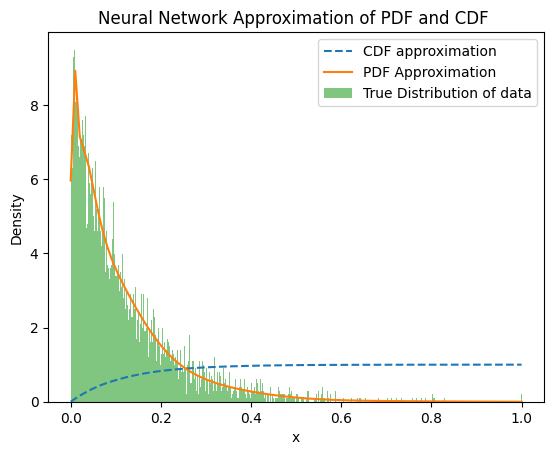
\includegraphics[width=\textwidth]{5ResultsDiscussion/pictures/MarginalTest/ExponentialHistogram.png}
            \subcaption*{(d) Exponential}
        \end{minipage}

    \vspace{1em}

    % --- (e) Laplace ---
        \begin{minipage}{0.45\textwidth}
            \centering
            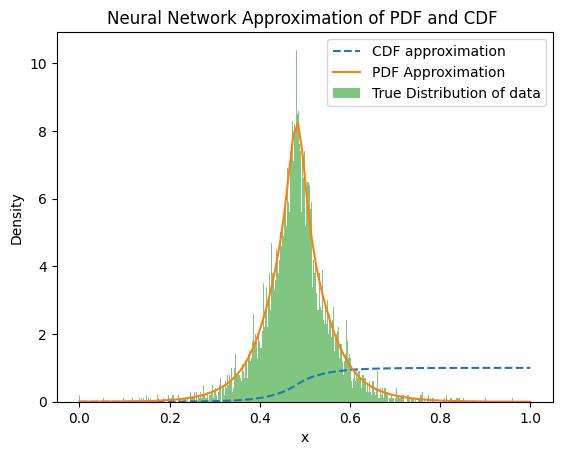
\includegraphics[width=\textwidth]{5ResultsDiscussion/pictures/MarginalTest/LaplaceHistogram.png}
            \subcaption*{(e) Laplace}
        \end{minipage}
    \hfill
    % --- (f) Lognormal ---
        \begin{minipage}{0.45\textwidth}
            \centering
            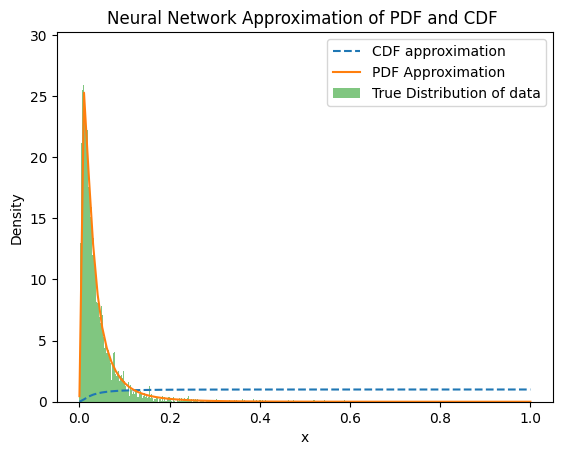
\includegraphics[width=\textwidth]{5ResultsDiscussion/pictures/MarginalTest/LognormalHistogram.png}
            \subcaption*{(f) Lognormal}
        \end{minipage}

    \caption{Marginal distribution visualizations. Each subfigure (a--f) shows a histogram with the trained model for the distribution.}
    \label{fig:MarginalResults}
\end{figure}


%%%%%%%%%%%%%%%%%%%%%%%%%%%%%%%%%%%%%%%%%%%%%%%%%%%%%%
%% Neural Copula Test   
%%%%%%%%%%%%%%%%%%%%%%%%%%%%%%%%%%%%%%%%%%%%%%%%%%%%%%
\subsection{Neural Copula Test}
The results of the grid search for the hyperparameters and weights are shown in \Cref{tab:Best_hyperparams} and \Cref{tab:Best_weights} respectively. Additionally, the losses for the different datasets using the best hyper parameters and weights are shown in \Cref{tab:LossesBestParameters}. These hyperparameter options answer the second research question \RQtwo about how to train the \gls{NC} to obtain the best results. The observations from these results are that the best performing hyperparameters are a network with three layers and ten neurons in each layer. The learning rate is 0.1 and the solver is Adam. The best performing scheduler is exponential and the number of epochs is 10000. 

\begin{table}[h!]
    \centering
    \caption{The best choice of hyper parameters found in the grid search.}
    \begin{tabular}{ll}
    \textbf{Hyperparameter} & \textbf{Options} \\
    \hline
    Network layers & 3 \\
    Network neurons & 10 \\
    Learning rate & 0.1 \\
    Scheduler & exponential \\
    Solver & Adam \\
    Epochs & 10000 \\
    Batch size & 2048 (Not valid, should remove this as dataset was smaller)\\
    \end{tabular}
    \label{tab:Best_hyperparams}
\end{table}
    
\begin{table}[h!]
    \centering
    \caption{The best choice of weights found for the copula loss function linear combination defined in \Cref{sec:NeuralCopulaLoss}.}
    \begin{tabular}{ll}
    \textbf{Weight} & \textbf{Options} \\
    \hline
    $\lambda_1$ & 1 \\
    $\lambda_2$ & 2 \\
    $\lambda_3$ & 0.5 \\
    $\lambda_4$ & 1 \\
    $\lambda_5$ & 1 \\
    \end{tabular}
    \label{tab:Best_weights}
\end{table}
    

    
\begin{table}[h!]
    \centering
    \caption{Losses for the datasets using the best hyper parameters and weights.}
    \begin{tabular}{lllllll}
        \textbf{Dataset} & \textbf{L1}& \textbf{L2}& \textbf{L3}& \textbf{L4}& \textbf{L5}& \textbf{Total Loss} \\
        \midrule
        Independent & 0.065705 & 0.025223 & 0.045032 & 0.077263 & 0.005574 & 0.218797 \\
        PositiveDependence & 0.290332 & 0.033420 & 0.049284 & 0.239172 & 0.017931 & 0.630140 \\
        NegativeDependence & -0.281669 & 0.025645 & 0.047584 & 0.082656 & 0.005116 & -0.120667 \\
        FrechetUpper & -3.846874 & 0.095704 & 0.257008 & 0.122417 & 0.014359 & -3.357385 \\
        FrechetLower & -3.611439 & 0.080854 & 0.000004 & 0.108494 & 0.003596 & -3.418491 \\
        \end{tabular}
    \label{tab:LossesBestParameters}
\end{table}

\begin{remark}
    When testing to rerun the training of the \gls{NC} for the different datasets a numerical instability was encountered. This sometimes results in that the copula does not train properly and that the loss function does not converge to zero for the constraint terms. In the cases where this was encountered the resulting copula surface did not look remotely like a copula function. 
\end{remark}

These results are limited to the datasets used in this test and the hyperparameters tested. The results may not be generalizable to other datasets or hyperparameters particularly when the dimensionality of the data increases. The results could also be influenced by the numerical instability observed during training. To be more certain about the results, it would be a good idea to test running this test with more hyperparameters, weights, and to run each training of the copulas several times to see which hyperparameters are truly the most reliable. This was not done in this thesis due to the large amount of time this would take to run. Given that this is a new method there is not much previous research to compare the results to.  


%%%%%%%%%%%%%%%%%%%%%%%%%%%%%%%%%%%%%%%%%%%%%%%%%%%%%
%% Portfolio Test
%%%%%%%%%%%%%%%%%%%%%%%%%%%%%%%%%%%%%%%%%%%%%%%%%%%%%
\subsection{Portfolio Test}
The results of the portfolio test are shown in \Cref{tab:DistributionDistances}. In the table, the distance between the data generated using the fitted copula and the true distribution is shown. The distance is calculated as described in \Cref{sec:GoodnessOfFit}. The last row in the table shows the total distance over all datasets for each copula used for fitting. This shows that the Gaussian copula was the best performing copula overall. The order of the remaining copulas is as follows: Clayton, Neural, and Students $t$. Of particular interest is the performance of the \gls{NC}. It seems like the \gls{NC} is not able to fit the data better than the other copulas as asked in \RQthree. 

\begin{table}[h!]
    \centering
    \caption{Distance between the fitted copula and the true distribution for the different distributions. The distance is calculated as described in \Cref{sec:GoodnessOfFit}.}
    \begin{tabular}{lllll}
    \textbf{Dataset/Copula} & \textbf{Gaussian} & \textbf{Students} & \textbf{Clayton} & \textbf{Neural} \\
    \hline
    % Gaussian, $\rho$: 0 & 0.00036880264225801646 & 0.0038564860944720883 & 0.00025453304967998163 & 0.002076942666237979 \\
    % Gaussian, $\rho$: 0.7 & 0.0005745609625385594 & 0.003405384070244613 & 0.0010251930676579886 & 0.0026765474087561796 \\
    % Students $t$, $\rho$: -0.8, $\nu$: 3 & 0.0005848558576855685 & 0.0013683433848652698 & 0.004119685177811808 & 0.0008999958003606833 \\
    % Clayton, $\alpha$: 4 &  0.0012345696582828495 & 0.0011805210541269663 & 0.001246438499213834 & 0.0026185757619811086 \\
    % Total & 0.0027627891207649942 & 0.009876652048795806 & 0.0038945080014170744 & 0.00827206163733595 \\
    Gaussian, $\rho$: 0               & 0.000369 & 0.003856 & 0.000255 & 0.002077 \\
    Gaussian, $\rho$: 0.7             & 0.000575 & 0.003405 & 0.001025 & 0.002677 \\
    Students $t$, $\rho$: -0.8, $\nu$: 3 & 0.000585 & 0.001368 & 0.004120 & 0.000900 \\ 
    Clayton, $\alpha$: 4              & 0.001235 & 0.001181 & 0.001246 & 0.002619 \\ %done
    \textbf{Total}      & \textbf{0.002764} & \textbf{0.009810} & \textbf{0.006646} & \textbf{0.008273} \\
    \end{tabular}
    \label{tab:DistributionDistances}
\end{table}

To better understand the results of the portfolio test, we investigate the data that the fitted copulas have generated. The data generated from the portfolio having dependence specified by a Clayton copula with $\alpha=4$ is shown in \Cref{fig:GeneratedDataClayton}. The figure shows the generated from each copula after being fitted to the data. We can see that it is only the clayton copula that is able to generate data that looks like the true distribution. Both the gaussian and the students $t$ are unable to capture the behavior of the data in the lower tail and hence the generated data looks very different from the true distribution. The \gls{NC} does seem to partially capture the behavior of the data by having a slightly pointy shape in the main body of the generated data similar to the true distribution also have. It does however have a very clear issue in that there are chunks of data that lie far from the true distribution. Given these observations it seems odd that the distance measure is similar for the Clayton, Gaussian, and Students $t$ copulas in \Cref{tab:DistributionDistances}. 

\begin{figure}
    \centering
    \begin{minipage}{0.4\textwidth}
        \centering
        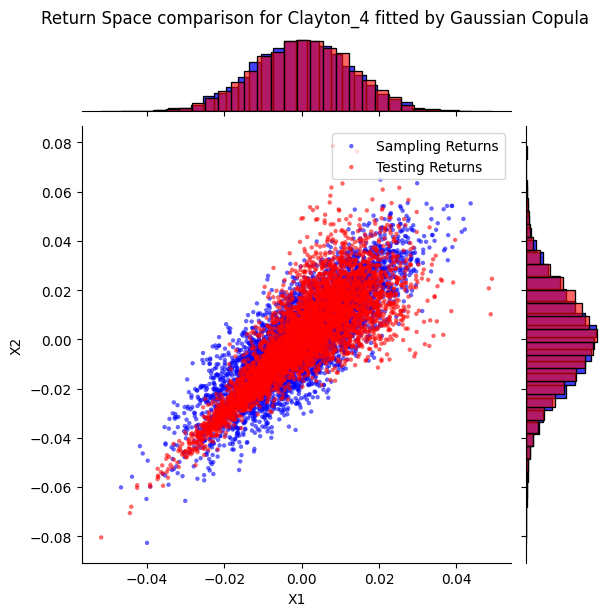
\includegraphics[width=\textwidth]{5ResultsDiscussion/pictures/PortfolioTest/ResultPortfolio4Gauss.png}
        \subcaption*{Gaussian copula}
    \end{minipage}
    \hfill
    \begin{minipage}{0.4\textwidth}
        \centering
        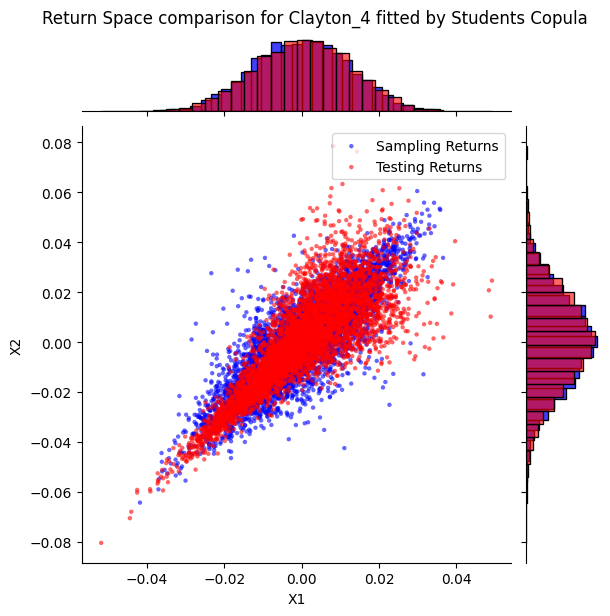
\includegraphics[width=\textwidth]{5ResultsDiscussion/pictures/PortfolioTest/ResultPortfolio4Students.png}
        \subcaption*{Students $t$ copula}
    \end{minipage}
    \vfill
    \begin{minipage}{0.4\textwidth}
        \centering
        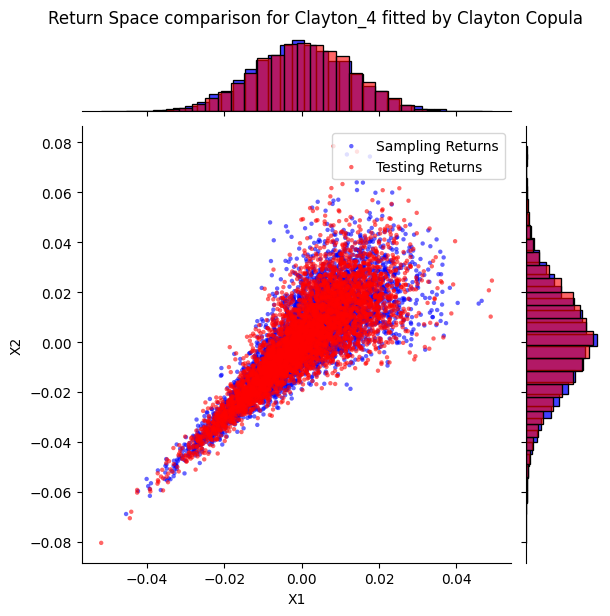
\includegraphics[width=\textwidth]{5ResultsDiscussion/pictures/PortfolioTest/ResultPortfolio4Clayton.png}
        \subcaption*{Clayton copula}
    \end{minipage}
    \hfill
    \begin{minipage}{0.4\textwidth}
        \centering
        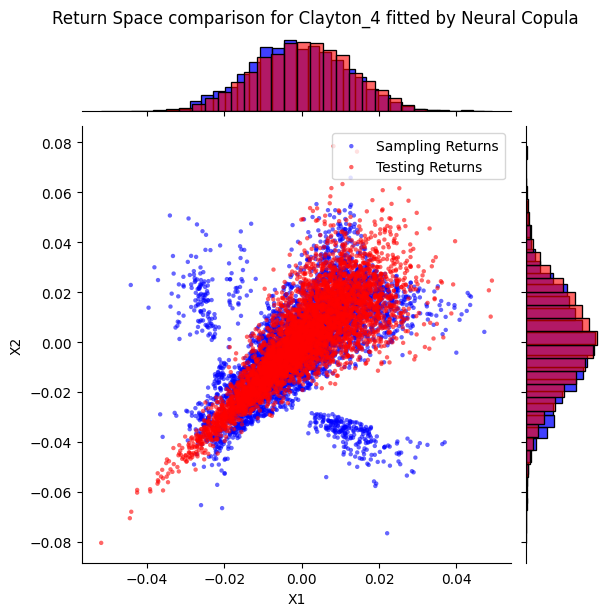
\includegraphics[width=\textwidth]{5ResultsDiscussion/pictures/PortfolioTest/ResultPortfolio4Neural.png}
        \subcaption*{Neural copula}
    \end{minipage}
    \caption{Fitted neural copula surfaces for Clayton $\alpha=4$ portfolio .}
    \label{fig:GeneratedDataClayton}
\end{figure}

The other portfolios are analyzed in a similar manner. The resulting figures are however placed in the appendix in \Cref{sec:CopulaResultsData}. In the following we will summarize the most important observations from the analysis of the generated data. 

In \Cref{fig:GeneratedDataGaussian0} we can see that the copulas seem to do quite well in capturing the true dependence being the Gaussian copula with $\rho = 0$. The Gaussian copula is unsurprisingly able to capture the true distribution well. The students $t$ copula captures the approximate shape of the true distribution but it creates too many extreme values resulting in that the generated data seems to have higher variance. The Clayton copula is able to capture the true distribution well which is unsurpricing as the Clayton copula coincides with the independence copula when $\alpha $ approaches 0. The \gls{NC} data also seems okay at capturign the true distribution. It does however not look completely circular as the true distribution does. Looking at the distance measures in \Cref{tab:DistributionDistances} we can see that Clayton is the best performing copula closely followed by the Gaussian copula.  

In \Cref{fig:GeneratedDataGaussian07} the portfolio having Gaussian dependence with $\rho = 0.7$ it seems like only the Gaussian copula is able to capture the true distribution well. The students $t$ copula generates data that is very similar to the true distribution but it has a lot of extreme values. The Clayton copula struggles to capture the true distribution because it has the lower tail dependence that the test data does not have. The \gls{NC} deviates a lot from the true distribution and is not able to capture the true distribution. The distance measures in \Cref{tab:DistributionDistances} show that the Gaussian copula is the best performing followed by the Clayton, Neural, and Students in that order. 


\Cref{fig:GeneratedDataStudents} shows the data generated when the copulas are fitted to the data generated from a Student's $t$ copula with $\rho = -0.8 \; \mathrm{and} \; \nu = 3$. For this portfolio it looks like all but the Clayton copula work well. The Clayton copula is unable to capture the distribution because it has negative correlation. This is something that the Clayton copula is not able to handle. The \gls{NC} seems to have a systematic issue with generating too few values in the lowe left quadrant despite working quite well. Looking at the distance measures in \Cref{tab:DistributionDistances} we can see that the Gaussian copula performs best followed by the \gls{NC} Student's $t$ and Clayton copula in that order. It is surprising that the Student's $t$ copula performs so poorly given that it is the true distribution and that the figure looks so good. 


Some further investigation in the fitted \gls{NC}s for the different portfolios are included in the appendix in \Cref{sec:CopulaSurfacesPlots}. \Cref{fig:NeuralCopulaSurface} shows the fitted \gls{NC} for the different portfolios. All of the fitted \gls{NC}s look like copulas should look in broad terms. All of the copulas do however seem to increase slower in the upper corner, where both $u_1$ and $u_2$ are close to 1, than they do before that. The copula fitted to the Gaussian portfolio with $\rho = 0$ is flat in the lower tail where both $u_1$ and $u_2$ are close to 0. It should not be if thinking back to the independence copula illustrated in \Cref{fig:FrechetBounds}.      

To investigate why the \gls{NC} does not successfully reproduce data looking like the true distributions the copula densities were visualized. This is because the copula density is used to sample from the fitted copula and might influence the generated data. The copula densities are shown in \Cref{sec:CopulaGradientsPlots} in \Cref{fig:NeuralCopulaGradient}. In the figure we see that the copula densities are not very smooth. Also, it is negative in some places, particularly near the edges. The wiggly nature of the copula densities might be the reason why the \gls{NC} is not able to generate data looking like the true distribution. It can possibly explain why the data generated from the \gls{NC} is very unevenly spread out as seen for the Clayton portfolio in \Cref{fig:GeneratedDataClayton}. 

These results are limited to the datasets used in this test and the copulas tested. Given that these results are not as positive as the results obtained bu \Citet[postnote]{ZengWang2022} we also need to be careful about drawing conclusions from these results. In particular, we acknowledge the possibility that we could have made mistakes. The differing results could also be due to the fact that we are using a very different approach of fitting the copula when training the copula on return data looking more like traditional probability distributions. Another possible reason for the differing results could be that we are evaluating the copulas based on the data generated from the fitted copula. As seen previously in this section, this might be explained by the non-smoothness of the copula density. This is something that would not have been a problem with the same impact for the \Citet{ZengWang2022} as for this experiment. The problem with sampling from the fitted copula gives rise to the question of how the copula can be trained to be more smooth. One possible solution is to use a different loss function term that penalizes the copula density for being non-smooth. Some small tests of this was done but no meaningful progress was made. 




\todo{Randomness in results}
\todo{what use when}


